\title{Final for Calculus-Based Physics: Electricity and Magnetism}
\author{Dr. Jordan Hanson - Whittier College Dept. of Physics and Astronomy}
\date{\today}
\documentclass[10pt]{article}
\usepackage[a4paper, total={18cm, 27cm}]{geometry}
\usepackage{outlines}
\usepackage{graphicx}
\usepackage{amsmath}
\begin{document}
\maketitle

\section{Equations and constants}

\begin{enumerate}
\item Volume of a sphere: $V_s = \frac{4}{3}\pi r^3$.
\item Density, mass and volume: $m = \rho V$.
\item Charge density, charge and volume: $Q = \rho V$.
\item Coulomb force: $\vec{F}_C = k \frac{q_1 q_2}{r^2}\hat{r}$.
\item Definition of electric field: $\vec{F}_C = q\vec{E}$.
\item Definition of electric flux: $\phi_E = \vec{E} \cdot \vec{A}$.
\item Gauss' Law: $\phi_E = q_{enc}/\epsilon_0$. (Assumes field is uniform over the surface).
\item Voltage and electric field, one dimension, uniform field: $|E| = - \frac{\Delta V}{\Delta x}$.
\item Voltage and electric field, general case: $\vec{E} = -\nabla V$.
\item Ohm's Law: $V = IR$.
\item Electrical power: $P = IV = I^2 R = V^2/R$.
\item Magnetic dipole moment: $\vec{\mu} = I \vec{A}$, where $\vec{A}$ is the area vector.
\item Torque on a magnetic dipole: $\tau = \vec{\mu} \times \vec{B}$.
\item Definition of magnetic flux: $\phi_m = \vec{B} \cdot \vec{A}$.  The units are T m$^2$, which is called a Weber, or Wb.
\item Faraday's Law: $emf = -N \frac{d \phi}{d t}$
\item Faraday's Law using \textbf{Inductance}, M: $emf = -M \frac{dI}{dt}$.
\item Typically, we refer to \textit{mutual inductance} between two objects as $M$, and \textit{self inductance} as $L$.
\item Inductance of a solenoid: $L = \mu_0 n^2 V$
\item Magnetic permeability: $\mu_0 = 4\pi \times 10^{-7}$ T m A$^{-1}$
\item Units of inductance: V s A$^{-1}$, which is called a Henry, or H.
\item Coulomb constant: $k = 8.9876 \times 10^{9}$ N m$^2$ C$^{-2}$.
\item Fundamental charge: $q_e = 1.602 \times 10^{-19}$ C.
\end{enumerate}

\clearpage

\section{Exercises}

\begin{enumerate}
\item \textbf{Chapters 5-6: Electrostatics and Gauss' Law}
\begin{enumerate}
\item Two charges 3 $\mu$C and 12 $\mu$C are fixed 1 m apart, with the second one to the right. Find the magnitude and direction of the net force on a -2 nC charge when placed at the following locations: (a) halfway between the two (b) half a meter to the left of the left charge. \\ \\
a) 0.6 mN to the right.  b) 0.312 mN to the right. \\
\item Using Gauss' law, prove that the electric field a distance $r$ from an infinite line of charge with charge per unit length $\lambda$ is
\begin{equation}
\vec{E} = \frac{\lambda}{2\pi\epsilon_0 r} \hat{r}
\end{equation} \\ \\
Let $l$ be a segment of the line of charge, with total charge $q = \lambda l$. Applying Gauss' law yields:
\begin{align}
\phi_E &= \vec{E} \cdot \vec{A} = \frac{q_{enc}}{\epsilon_0} \\
q_{enc} &= \lambda l \\
\vec{E} \cdot \vec{A} &= EA \\
EA &= \frac{\lambda l}{\epsilon_0} \\
A &= 2\pi r l \\
E(2\pi r l) &= \frac{\lambda l}{\epsilon_0} \\
\vec{E} &= \frac{\lambda}{2\pi\epsilon_0 r} \hat{r}
\end{align}
The direction is given by symmetry (outward from the wire).
\end{enumerate}
\item \textbf{Chapters 7-8: Voltage and Capacitance}
\begin{enumerate}
\item The voltage across a capacitor is 100 mV, and the distance between the two charged surfaces is 1 mm.  What is the electric field in the capacitor? \\ \\
When the electric field is uniform, the field is given by the voltage divided by the distance: $E = \Delta V / \Delta x = 0.1/10^{-3}$ V/m, or 100 V/m. \\
\item An electric potential is defined by $V(x,y,z) = a x + b \sin(ky)$, with $a = 2.0$ V m$^{-2}$, $b = 1.0$ V m$^{-1}$, and $\omega = 10\pi$ rad m$^{-1}$.  What is the corresponding electric field at $P = (-1,1)$? \\ \\
The negative gradient gives you the electric field:
\begin{align}
\vec{E} = -\nabla V &= -\frac{\partial}{\partial x} (ax)\hat{x} - \frac{\partial}{\partial y} b\sin(ky)\hat{y} \\
\vec{E} &= -a\hat{x}-kb \cos(ky)\hat{y}
\end{align}
\end{enumerate}
\item \textbf{Chapters 9-10: Current, Resistance, and DC Circuits}
\begin{enumerate}
\item Two resistors are connected in series.  One has 1000$\Omega$ resistance, and the other has 500$\Omega$ resistance.  If the resistors are connected in series to a 1.5 V battery, (a) what current will flow? (b) Draw a graph of $I$ vs. $V$ in this system, as if $V$ could vary but the total resistance were fixed.  Label the axes of the graph and indicate the slope. \\ \\
The total resistance is 1500$\Omega$, because the resistors are in series.  Using Ohm's law, we have 1.5V/1500$\Omega$ = 1.0 mA.  The graph is a linear graph, and if we place Volts on the y-axis, and current on the x-axis, the slope will be 1500.  However, if we put current on the y-axis and volts on the x-axis, the slope will be 1/1500. \\
\item How much energy in kiloWatt hours does a $10\Omega$ light consume if it draws 1.0 Amp of current for 6 hours? \\ \\
The relevant equation is $P=IV = I^2 R$.  We have the current and the resistance, so this is a $1.0^2 \times 10.0 = 10.0$ W light bulb.  Thus, a 10W light running for 6 hours consumes 60 W hours of energy, or 0.06 kW hours.  Remember that energy $U = P \Delta t$, so a ``Watt hour'' or ``kW hour'' is an energy, not a power. \\
\begin{figure}
\centering
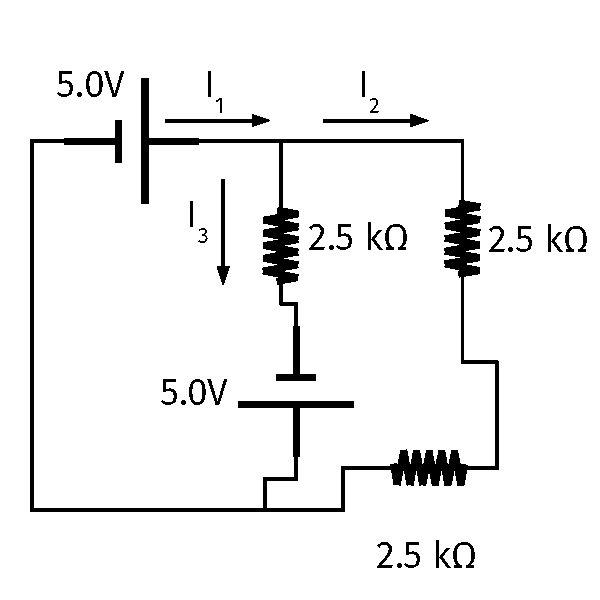
\includegraphics[width=0.4\textwidth]{iV2.pdf}
\caption{\label{fig:batt1} A circuit with two battery voltages and three resistors.}
\end{figure}
\item Solve for the currents in Fig. \ref{fig:batt1}.
\begin{itemize}
\item $I_1 = 5$ mA
\item $I_2 = 1$ mA
\item $I_3 = 4$ mA
\end{itemize}
\end{enumerate}
\item \textbf{Chapters 11-12: Magnetic fields and Sources of Magnetic Fields}
\begin{enumerate}
\item A circular loop of wire of area $10^{-1}$ m$^{2}$ carries a current of 1.0 A, and it is situated in the xy plane.  (a) An external 1.0 T B-field is applied in the positive z-direction.  What is the magnitude of the torque? (b) A magnetic field is applied in the x-direction.  What is the magnitude of the torque? \\ \\
(a) In the first case, the magnetic moment of the loop is in the +z direction, and so is the field, so the torque is zero.  (b) $|\vec{\tau}_m| = |\vec{\mu} \times \vec{B}| = \mu B\sin(\theta)$.  The angle is 90 degrees, so the torque is $\mu B = I A B = 1.0 10^{-1} 1.0 = 10^{-1}$ N m.
\end{enumerate}
\item \textbf{Chapters 13-14: Electromagnetic Induction and Inductance}
\begin{enumerate}
\item Two solenoids each have volume $V = 6 \times 10^{-6}$ m$^3$, and length $l = 2.0$ cm.  One has 1000 turns, and one has 100.  What is the inductance of each, in Henries? \\ \\
The formula in this case is $L = \mu_0 n^2 (V)$, so the smaller inductance is $4\pi \times 10^{-7} (0.5 \times 10^{4})^2 6 \times 10^{-6}$ H, so we have $L = 3\pi/50$ mH.  The larger one simply scales up because it has the same properties but 10 times the coils, so it should be 100 times the inductance, or $6\pi$ mH. \\
\item Suppose the current changes in the smaller inductor in the previous problem at a rate of $dI/dt = 100.0$ A s$^{-1}$.  (a) What is the emf induced in it?  (b) What is the emf induced in the larger inductor? \\ \\
We have
\begin{equation}
emf = -L \frac{dI}{dt} = - \frac{3\pi}{50} \times 10^{-3} \times 100.0 = - \frac{3\pi}{500}~~V
\end{equation}
Again, the larger inductor is larger by a factor of 100, so the induced emf should also be larger by that same factor.  We find $-\frac{3\pi}{5}$ V. \\
\item Suppose the two inductors were interleved, such that a current through one inductor would generate a solenoidal magnetic field that happened to pass through the other solenoid.  If a changing current is passed through the smaller inductor, which of the following is true of the larger?
\begin{itemize}
\item A: Nothing would happen: the emf is only induced in the first inductor.
\item B: An emf would be induced in the second inductor, equal to the emf in the first inductor.
\item C: An emf would be induced in the second inductor, but smaller than the emf in the first inductor.
\item D: An emf would be induced in the second inductor, but larger than the emf in the first inductor.
\end{itemize}
\textit{The answer is D, because the larger inductor sees the same flux as the smaller, but with more coils.  Thus, the induced emf is larger in the larger inductor.}
\end{enumerate}
\end{enumerate}

\end{document}